\begin{table}[bt]
	\rule{\linewidth}{2pt}
	\caption{selected beams section chosen from the Parker IPS catalogue \cite{parker-ds} and related main properties (area, moments of inertia and weight per unit length).}
	\label{tab:beamchoice}
	\rule{\linewidth}{1pt} \vspace{0mm}	
	
	\begin{center}
		\begin{tabular}{p{3cm} | c c c c  |  l }
			& Area & \multicolumn{2}{c}{Moments of inertia} & Weight \\
			Usage & $A [cm^2]$ & $I_{xx} [cm^4]$ & $I_{yy} [cm^4]$ & $p [kg/m]$ & Product code \\ \hline
			track & 9.29 & 14.26 & 14.26 & 2.53 & \texttt{11-040} \\
			supports & 5.20 & 8.27 & 8.27 & 1.41 & \texttt{10-540} \\
		\end{tabular}
	\end{center}
	
	\vspace{3mm}
	\rule{\linewidth}{1pt}
	{\scriptsize
		\begin{multicols}{2}
		\begin{center}
			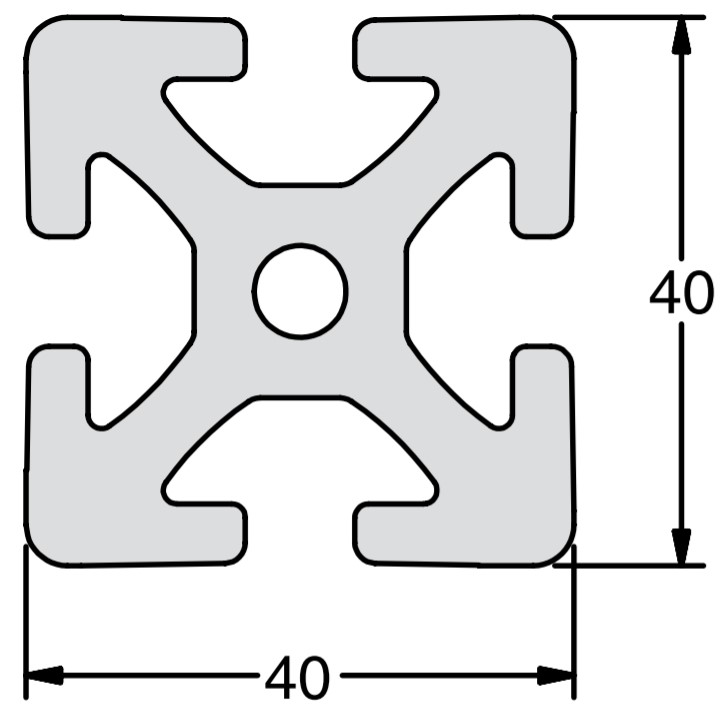
\includegraphics[height=2cm]{11-040}	\\		
			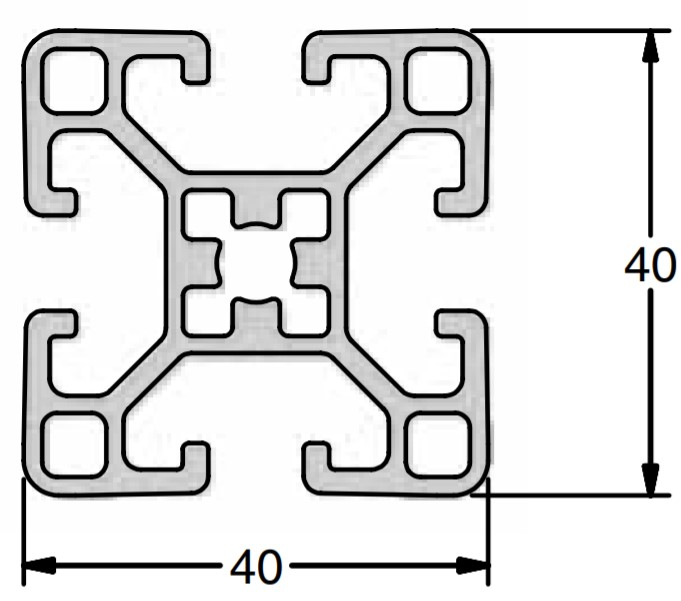
\includegraphics[height=2cm]{10-540}
		\end{center}
		\end{multicols}
		Representation of the sections for the track beam (on the left) and the supports (right).
	}	
	
	\rule{\linewidth}{2pt}
	
\end{table}